%----------------------------------------------------------------------------------------
%	PACKAGES AND THEMES
%----------------------------------------------------------------------------------------
\documentclass[aspectratio=169,xcolor=dvipsnames]{beamer}
\usetheme{General}

\usepackage{hyperref}
\usepackage{graphicx} % Allows including images
\graphicspath{ {./images/} }
\usepackage{booktabs} % Allows the use of \toprule, \midrule and \bottomrule in tables
\usepackage{multicol}

%----------------------------------------------------------------------------------------
%	TITLE PAGE
%----------------------------------------------------------------------------------------

\title[short title]{sCrypto} 
\subtitle{Crypto trading bot}


\institute[RiTeh] 
{
Sveučilište u Rijeci - Tehnički fakultet 
}
\date{29.03.2021} 


%----------------------------------------------------------------------------------------
%	PRESENTATION SLIDES
%----------------------------------------------------------------------------------------

\begin{document}

\begin{frame}
  \titlepage
\end{frame}

\begin{frame}{Tablica sadržaja}
  \tableofcontents
\end{frame}

%------------------------------------------------
\section{Tok rada}
%------------------------------------------------

\begin{frame}{Određivanje toka rada}
    \item Odabir platforme
    \item Odabir servera
    \item Planiranje i strategija
    \item Jednostavniji bot
    \item Složeniji bot
\end{frame}

%------------------------------------------------

%------------------------------------------------
\section{Izrada dijagrama}
%------------------------------------------------

\begin{frame}{WBS dijagram}
    \item Planiranje osnovnih funkcija 
    \item Podjela rada na manje cjeline radi bolje organizacije
    \begin{figure}
        \centering
        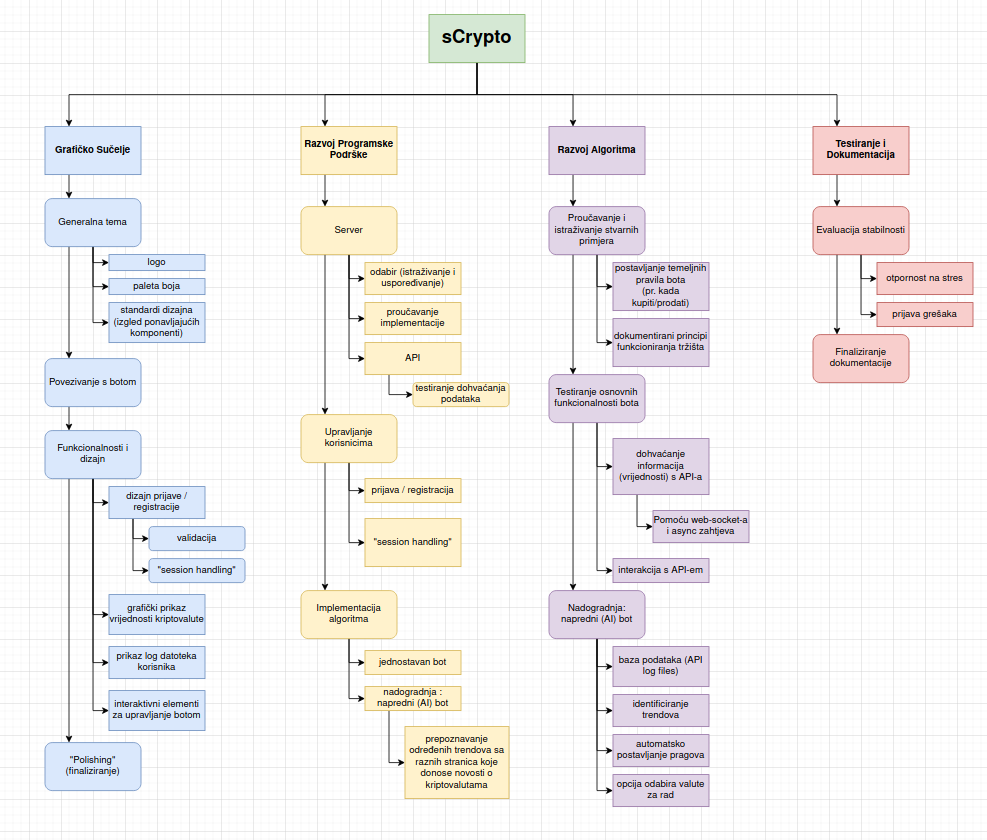
\includegraphics[width=7cm]{wbs}
        \caption{WBS dijagram}
        \label{fig:wbs}
    \end{figure}
\end{frame}

%------------------------------------------------

\begin{frame}{PERT dijagram}
    \item Određivanje zavisnosti zadataka 
    \item Vrijeme potrebno za izradu
    \item Dozvoljeno kašnjenje zadataka ne kritičnog puta
    
\end{frame}

\begin{frame}{PERT dijagram}
    \begin{figure}
        \centering
        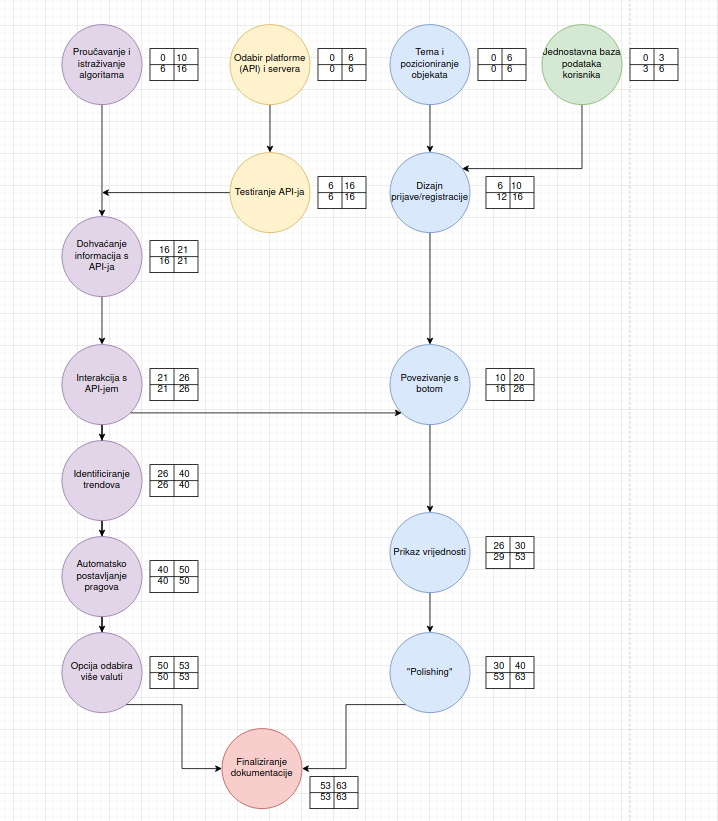
\includegraphics[width=6cm]{pert}
        \caption{Pert diagram}
        \label{fig:pert}
    \end{figure}
\end{frame}

%------------------------------------------------
\section{Platfomra i server}
%------------------------------------------------

\begin{frame}{Odabir platforme}
    \item Pronalazak platformi 
    \item Usporedba 
    \item Odabir
\end{frame}

%------------------------------------------------

\begin{frame}{Odabir servera}
    \item Pronalazak pogodnih solucija
    \item Odlučivanje za cloud based server
    \item Pronalazak servera
    \item Usporedba
    \item Odabir
\end{frame}

%------------------------------------------------
\section{Strategija}
%------------------------------------------------

\begin{frame}{Strategija}
    \item Odabir kriptovalute
    \item Spot vs. leverage trgovanje
    \item Indikatori tehničke analiza
    \item Strategije trgovanja temeljene na indikatorima tehničke analize
    \item Odabir
    
\end{frame}

%------------------------------------------------
\section{Izrada bota}
%------------------------------------------------

\begin{frame}{Jednostavan bot}
    \item 2 osnovna stanja kupi i prodaj
    \item ručno određivanje pragova
    \item odabir valute
    \item osnovna komunikacija s API-jem
\end{frame}

%------------------------------------------------

\begin{frame}{Složeni bot}
  \item AI
  \item automatsko određivanje pragova
  \item provjera stranica s trendovima
  \item napredniji GUI
  \item limitirani nalozi
\end{frame}

%------------------------------------------------

\begin{frame}{Dokumentacija}
    \item Tema: Bot za trgovinu kriptovalutama
    \item GitHub https://github.com/MSrica/sCrypto
    \item Članovi: Fran Grenko, Deni Klen, Ani Perušić, Mateo Srića, Karlo Veršić
\end{frame}
%------------------------------------------------

\end{document}